% This is a sample LaTeX input file.  (Version of 11 April 1994.)
%
% A '%' character causes TeX to ignore all remaining text on the line,
% and is used for comments like this one.

\documentclass[11pt]{article}      % Specifies the document class
\usepackage{amsfonts,amssymb,amsmath}
\topmargin-0.2in
\textheight9.0in
\oddsidemargin-0.2in
\evensidemargin-0.2in
\textwidth6.5in

\usepackage{graphicx} % Required for inserting images
\usepackage{booktabs}
\usepackage{subcaption}
\usepackage{xcolor}  

\usepackage{listings}
\lstset{
	basicstyle=\footnotesize\ttfamily,
	columns=flexible,
	breaklines=true,
	commentstyle=\color{red},
	keywordstyle=\color{black}\bfseries}

\newcommand{\mZ}{\mathbb Z}
\newcommand{\mR}{\mathbb R}
\newcommand{\mC}{\mathbb C}
\newcommand{\mQ}{\mathbb Q}
\newcommand{\ep}{\epsilon}
\begin{document}             % End of preamble and beginning of text.

%\thispagestyle{empty}
\begin{center}
{\bf\large HW2(FEA): Appiah Francis}\\
\vspace{0.05in}
\end{center}
%--- coding
\begin{enumerate}
\item[(iii)] The code is Implemented with a uniform mesh $h_j = h = \frac{1}{N+1}$. From (i) the exact solution is given by 
$$u(x) = \frac{e^{1/\varepsilon}}{e^{1/\varepsilon} - 1} - \frac{e^{1/\varepsilon}}{e^{1/\varepsilon} - 1} e^{x/\varepsilon}$$ with it's  derivative 
$$u'(x) =  -\frac{1}{\varepsilon} \frac{e^{1/\varepsilon}}{e^{1/\varepsilon} - 1} e^{x/\varepsilon}.$$
Below is the plot of the exact solution againts the approximate solution $U_I(x)$.
\begin{figure}[htbp]
	\centering
	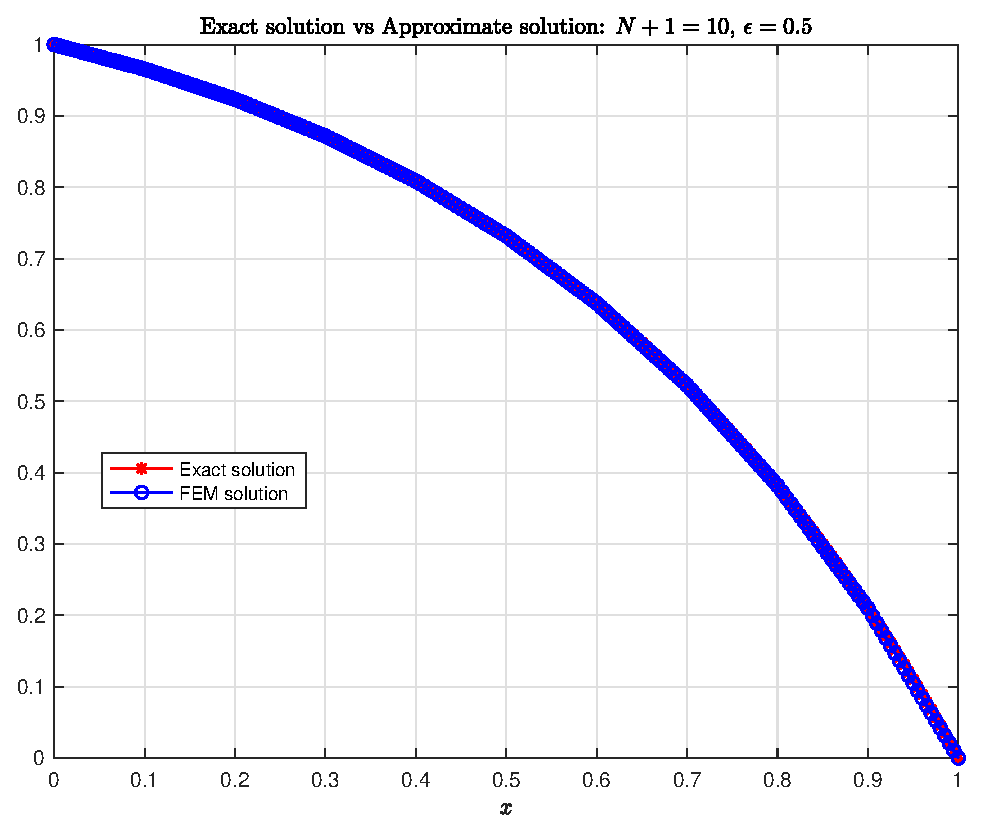
\includegraphics[width=0.55\textwidth]{img/solplot_N10_eps0.5.eps}
	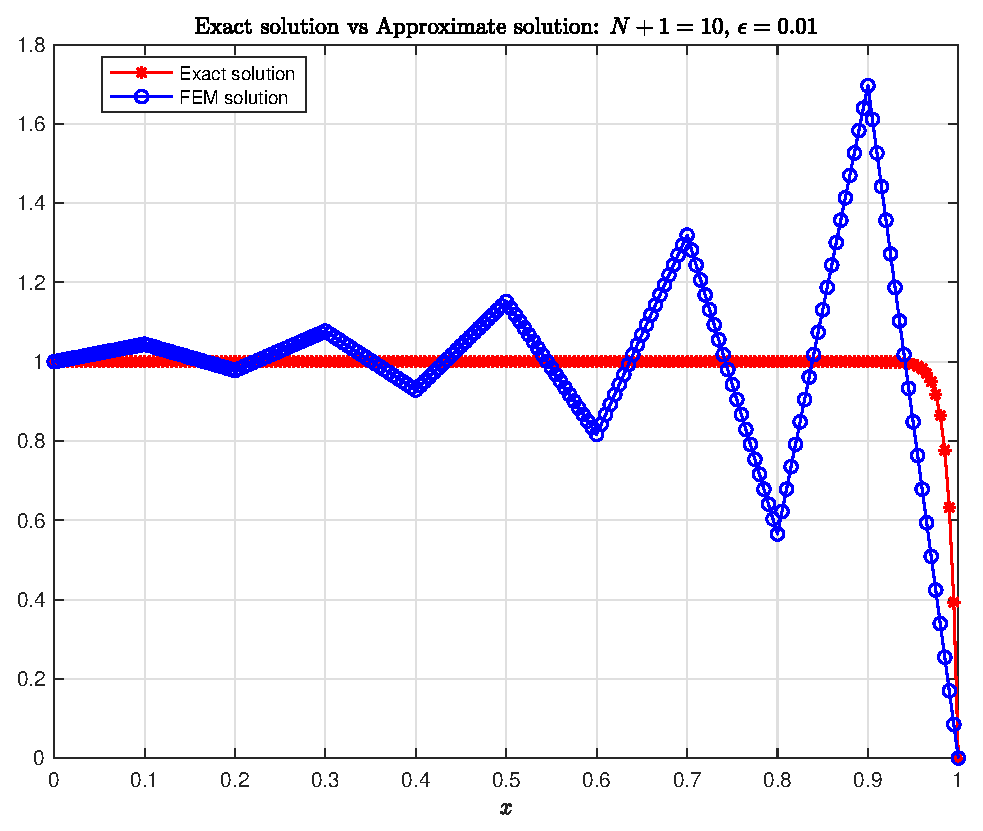
\includegraphics[width=0.55\textwidth]{img/solplot_N10_eps0.01.eps}
	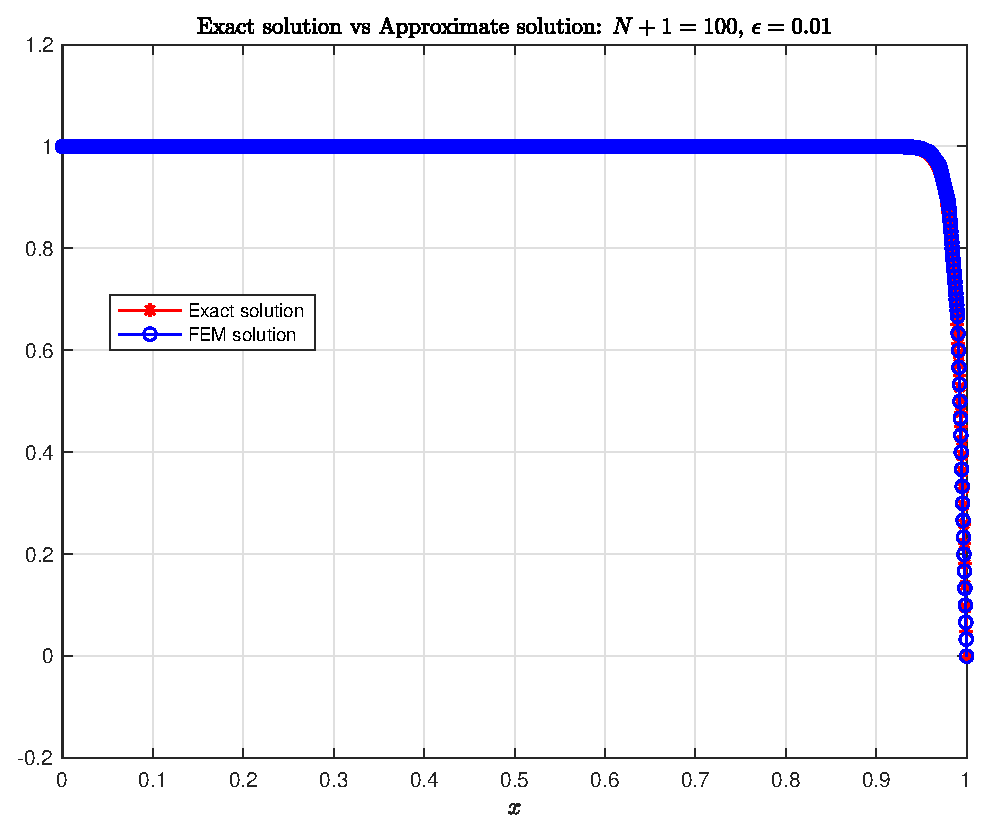
\includegraphics[width=0.55\textwidth]{img/solplot_N100_eps0.01.eps}
	\label{fig:N3}
\end{figure}
\begin{table}[!h]
	\caption{Errors and convergence orders when $\varepsilon = 0.5$}
	\vspace{0.1in}
	\centering
	\begin{tabular}{|c|c|c|c|c|}
		\hline
		$N+1$ & $||e_h(\cdot)||_{L^2([0,1])}$ & Order & $||e_h(\cdot)||_{H^1([0,1])}$ & Order \\
		\hline
		10    & 1.77E-03 & -    & 7.46E-02 & - \\
		100   & 1.77E-05 & 2.00 & 7.33E-03 & 1.01 \\
		1000  & 1.77E-07 & 2.00 & 7.32E-04 & 1.00 \\
		10000 & 1.77E-09 & 2.00 & 7.31E-05 & 1.00 \\
		\hline
	\end{tabular}
	\label{tab1}
\end{table}

\begin{table}[!h]
	\caption{Errors and convergence orders when $\varepsilon = 0.01$}
	\vspace{0.1in}
	\centering
	\begin{tabular}{|c|c|c|c|c|}
		\hline
		$N+1$ & $||e_h(\cdot)||_{L^2([0,1])}$ & Order & $||e_h(\cdot)||_{H^1([0,1])}$ & Order \\
		\hline
		10    & 2.01E-01 & -    & 1.64E+01 & - \\
		100   & 5.10E-03 & 1.59 & 2.35E+00 & 0.84 \\
		1000  & 5.26E-05 & 1.99 & 2.27E-01 & 1.02 \\
		10000 & 5.26E-07 & 2.00 & 2.26E-02 & 1.00 \\
		\hline
	\end{tabular}
	\label{tab_eps001}
\end{table}

\begin{table}[!h]
	\caption{Errors and convergence orders when $\varepsilon = 0.001$}
	\vspace{0.1in}
	\centering
	\begin{tabular}{|c|c|c|c|c|}
		\hline
		$N+1$ & $||e_h(\cdot)||_{L^2([0,1])}$ & Order & $||e_h(\cdot)||_{H^1([0,1])}$ & Order \\
		\hline
		10    & 2.59E+00 & -    & 1.79E+02 & - \\
		100   & 6.19E-02 & 1.62 & 5.18E+01 & 0.54 \\
		1000  & 1.61E-03 & 1.58 & 7.45E+00 & 0.84 \\
		10000 & 1.66E-05 & 1.99 & 7.18E-01 & 1.02 \\
		\hline
	\end{tabular}
	\label{tab_eps0001}
\end{table}
\clearpage
\section{Conclusion}
When $\varepsilon = 0.5$ the diffusion part dominates, and the solution is smooth across the domain. Using a uniform mesh works well for all values of $N+1$. We can see from the table the $L^2$ norm and $H^1$ norm convergence is 2nd and 1st order respectively. This is consistent with the theoretical error estimates for piecewise linear finite element methods.   When $\varepsilon$ is very small, the equation behaves approximately like $u'(x) = 0$, which gives a constant solution. For most of the domain $x<1$, the solution satisfies
\[
u(x) \approx 1.
\]
However, near $x=1$, the solution rapidly decreases to satisfy the boundary
condition $u(1)=0$.  A uniform mesh may not
resolve this layer unless the mesh size satisfies $h \ll \varepsilon$. The convergence rates deteriorate initially
because the uniform mesh cannot adequately resolve this issue.  The error is largest near x =1, where the solution has steep gradients. This steep gradients creates very large derivatives. This is evident from table 2 and 3 as the $H^1$ norm errors are huge when the mesh is not refined enough. For $\varepsilon = 0.01$ and $N+1 = 10$ we see FEM struggles to approximate the exact solutionn, but 
as the mesh is refined, the error decreases and the expected convergence
rates are eventually recovered.
The convection--diffusion problem demonstrates the challenges of solving
singularly perturbed equations numerically. When $\varepsilon$ is small, the
solution develops a boundary layer(perturbation methods), which requires
fine mesh resolution for accurate approximation. 
\end{enumerate}
\lstinputlisting[language=matlab, numbers=left, stepnumber=1, firstline=1,caption={main.m },label=code:main1,frame=single]{main.m}
\lstinputlisting[language=matlab, numbers=left, stepnumber=1, firstline=1,caption={twoPointBVP.m },label=code:main2,frame=single]{twoPointBVP.m}
\lstinputlisting[language=matlab, numbers=left, stepnumber=1, firstline=1,caption={formMatrix.m },label=code:main3,frame=single]{formMatrix.m}
\lstinputlisting[language=matlab, numbers=left, stepnumber=1, firstline=1,caption={$U_h (x)$ function },label=code:main4,frame=single]{UhFunc.m}
\lstinputlisting[language=matlab, numbers=left, stepnumber=1, firstline=1,caption={$U'_h(x)$ function },label=code:main5,frame=single]{UhFuncx.m}
\end{document}               % End of document.
